\section{Transmissionsledningar}
\label{transmissionsledningar}
\index{transmissionsledning}

En matarledning ska med så små förluster som möjligt överföra den
högfrekventa energin från sändaren fram till sändarantennen.
Omvänt ska den energi som fångats upp av mottagarantennen transporteras
till mottagaren med så små förluster som möjligt.

\subsection{Avstämd matarledning}
\index{transmissionsledning!avstämd}

\subsubsection{Spännings- och strömkoppling}

\begin{wrapfigure}[17]{R}{0.5\textwidth}
  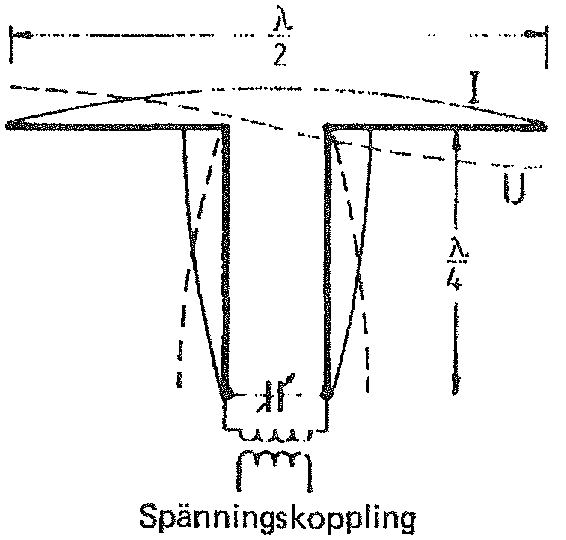
\includegraphics[width=0.5\textwidth]{images/cropped_pdfs/bild_2_6-21.pdf}
  \caption{Spänningskopplad $\lambda/2$-dipol}
  \label{fig:bildII6-21}
\end{wrapfigure}

Bild \ref{fig:bildII6-21} visar en \(\lambda/2\)-dipol som kopplas till
sändarutgången via en \(\lambda/4\) matarledning.
För tydlighetens skull visas ledningen som en bandkabel.

Vid sändning uppstår en stående våg på matarledningen och på dipolen.
Även matarledningen svänger med och är avstämd till resonans
-- därav namnet avstämd matarledning.

Vi följer ström- och spänningsfördelningen bakåt från dipolen till
sändaren och finner följande:

I vardera änden av \(\lambda/2\)-dipolen uppträder en spänningsbuk (streckade
linjer) och i mitten av dipolen uppträder en strömbuk (heldragna linjer).
Den stående vågen, med strömbuken på dipolens mitt, fortsätter ner på
\(\lambda/4\)-matarledningen.
I nedre änden av matarledningen vid sändarutgången har det uppstått en strömnod
och en spänningsbuk, vilket innebär att matarledningen ska spänningskopplas
till sändaren.

\begin{wrapfigure}[19]{R}{0.5\textwidth}
  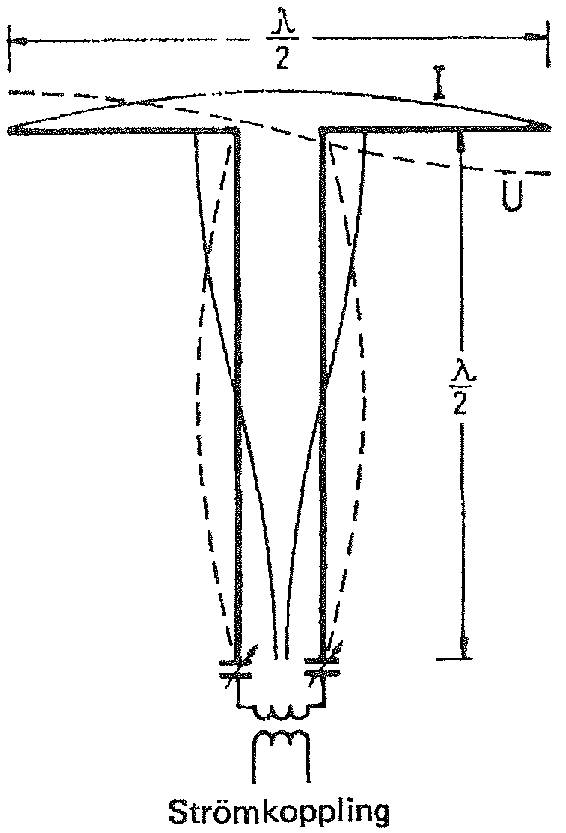
\includegraphics[width=0.5\textwidth]{images/cropped_pdfs/bild_2_6-22.pdf}
  \caption{Strömkopplad $\lambda/2$-dipol}
  \label{fig:bildII6-22}
\end{wrapfigure}

Om matarledningen i stället är \(\lambda/2\) lång, så uppstår i
stället en spänningsnod och en strömbuk i nedre änden av ledningen,
vilket innebär att matarledningen ska strömkopplas till sändaren,
vilket visas i bild \ref{fig:bildII6-22}.

Ström- och spänningsfördelningen kan ritas upp för en \(\lambda\)-dipol resp.
\(\lambda/2\)-dipol i kombination med matarledningar med längderna
\(n \cdot \lambda/4\) (med \(n\) = 1, 2, 3 \dots).
Med hjälp av teckningen kan man avgöra om ström- eller spänningskoppling måste
användas.

\begin{figure}
  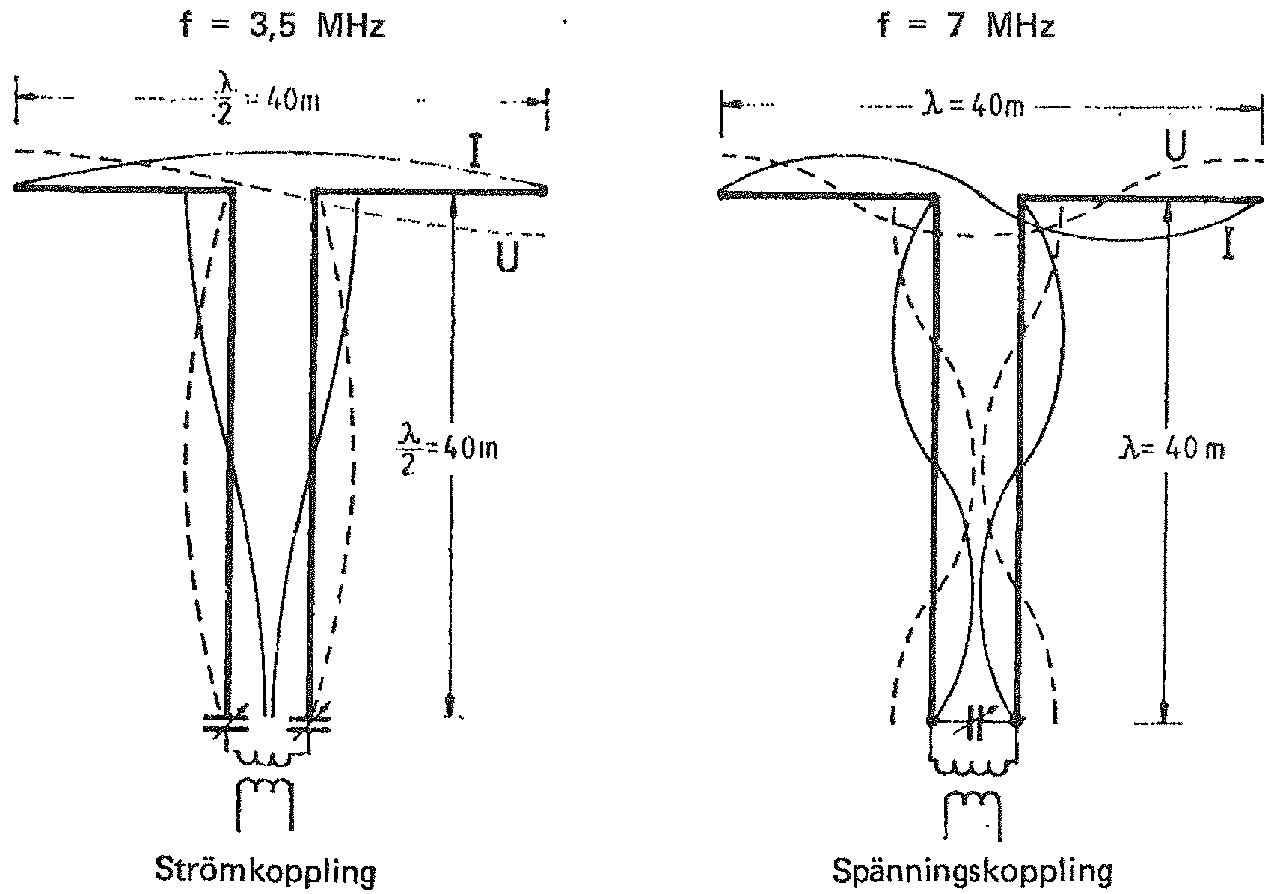
\includegraphics[width=\textwidth]{images/cropped_pdfs/bild_2_6-23.pdf}
  \caption{Samma $\lambda/2$-dipol på grundfrekvensen respektive 1:a övertonen}
  \label{fig:bildII6-23}
\end{figure}

Bild \ref{fig:bildII6-23} visar en \(\lambda/2\)-dipol för 80~m-bandet ansluts
till en avstämd matarledning med längden \(\lambda/2 = 40\) m.

Önskar man använda denna dipol för 80~m-bandet på 40-, 20- och 10~m-banden
måste en s.k. antennkopplare anslutas mellan sändaren och matarledningen.
Kopplaren har alltid strömmatad ingång och valmöjlighet för ström- respektive
spänningsmatad utgång.
Se om antennkopplare sist i detta kapitel.

\subsection{Oavstämd matarledning}
\index{transmissionsledning!oavstämd}

Begreppet ''oavstämd'' syftar på ledningslängden, som under vissa
bestämda förutsättningar kan vara godtyckligt lång.
I motsats till den avstämda matarledningen behöver ledningslängden på en
oavstämd matarledning inte stå i förhållande till våglängden \(\lambda\).
Som matarledning kan användas en koaxialkabel eller öppen transmissionsledning.

\textbf{Fördelar:}
Enkel uppbyggnad, mindre kritisk kabelföring och längden kan väljas godtyckligt.

\textbf{Nackdelar:}
Sändaren, matarledningen och antennen måste alltid vara impedansanpassade till
varandra.
Dessutom måste antenn- och kabelströmmarna balanseras.
I det följande visas hur dessa krav kan uppfyllas.

Som matarledning upp till mikrovågsområdet är koaxialkabeln vanligast.

\subsection{Koaxialkabel}
\textbf{
HAREC a.\ref{HAREC.a.6.3.2}\label{myHAREC.a.6.3.2}
}
\index{koaxialkabel}
\index{transmissionsledning!koaxial}

\begin{wrapfigure}{R}{0.5\textwidth}
  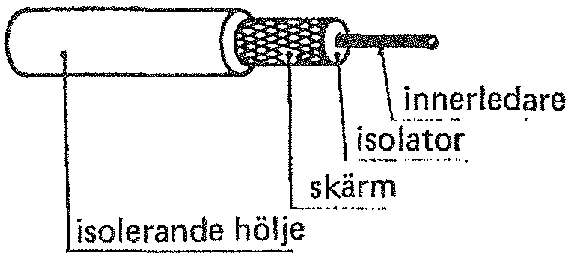
\includegraphics[width=0.5\textwidth]{images/cropped_pdfs/bild_2_6-24.pdf}
  \caption{Koaxialkabel}
  \label{fig:bildII6-24}
\end{wrapfigure}

Koaxialkabelns uppbyggnad framgår av bild \ref{fig:bildII6-24}.
I en koaxialkabel bildas ett radiellt elektriskt fält mellan mittledaren och
insidan av ytterledaren.
Av strömmen bildas också ett magnetiskt koncentriskt fält mellan inner- och
ytterledaren.
Resultatet blir ett elektromagnetiskt fält, som breder ut sig i kabeln som en
TEM-våg (TE-våg = transversell elektrisk, TM-våg = transversell magnetisk och
TEM-våg = transversell elektromagnetisk våg).

Koaxialkabeln består av en isolerad innerledare omgiven av en ytterledare, vars
insida är kabelns andra strömledare.
Ytterledaren förhindrar dessutom HF-utstrålning och inkommande störningar.
I motsats till den symmetriskt uppbyggda bandkabeln, tillhör
koaxialkabeln de osymmetriska ledningarna.

Vanliga karakteristiska impedanser för koaxialkabel är 50 och 75~\(\Omega\).

\subsection{Bandkabel}
\textbf{
HAREC a.\ref{HAREC.a.6.3.1}\label{myHAREC.a.6.3.1}
}
\index{bandkabel}
\index{transmissionsledning!bandkabel}

\begin{wrapfigure}{R}{0.5\textwidth}
  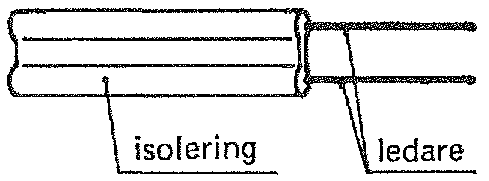
\includegraphics[width=0.5\textwidth]{images/cropped_pdfs/bild_2_6-25.pdf}
  \caption{Bandkabel}
  \label{fig:bildII6-25}
\end{wrapfigure}

Som framgår av bild \ref{fig:bildII6-25} består bandkabeln av två parallella
ledare med samma dimensioner.
Kabelns isolering håller samtidigt ledaravståndet rätt.
I ett kraftigare utförande övergår denna ledningstyp till att bestå av ett
ledarpar med isolerade spridare på jämna avstånd.
Den kommer att likna en stege det ursprungliga utförandet på en matarledning.

Vanliga karakteristiska impedanser för bandkabel är 75 och 300~\(\Omega\).

\subsection{Vågledare}
\textbf{
HAREC a.\ref{HAREC.a.6.3.3}\label{myHAREC.a.6.3.3}
}
\index{vågledare}
\index{transmissionsledning!vågledare}

Inom mikrovågsområdet är den vanligaste typen av matarledning
s.k. vågledare som saknar mittledare.
I en vågledare däremot, matas energin fram enbart som speciella elektriska och
magnetiska fält (TEM) i mönster som kallas moder.

\subsection{Hastighetsfaktor}
\textbf{
HAREC a.\ref{HAREC.a.6.3.5}\label{myHAREC.a.6.3.5}
}
\index{transmissionsledning!hastighetsfaktor}

Vid bestämning av den mekaniska längden på en matarledning måste
hänsyn tas till att våghastigheten längs ledningen är lägre än ljushastigheten.
Man talar om en hastighetsfaktor relativt ljushastigheten.
Hastighetsfaktorn beror på ledningens utförande och ingående material.

En koaxialkabel har hastighetsfaktorn \(v = \frac{1}{\sqrt{\varepsilon}}\),
där \(\varepsilon\) är den relativa dielektricitetskonstanten i
isolationsskiktet.
Ett vanligt förekommande isolationsmaterial i koaxialkablar är polyetylen med
dielektricitetskonstanten \(\varepsilon = 2,25\).
Hastighetsfaktorn \(v\) (velocity factor) blir då

\[
v = \frac{1}{\sqrt{\varepsilon}} = \frac{1}{\sqrt{2.25}} = \frac{1}{1,5} = 0,666
\]

1~meter av en sådan koaxialkabel är \(1/0,666 = 1,333\) meter för en HF-signal.
Även bandkablar har naturligtvis en hastighetsfaktor, vanligen 0,7--0,85.

\subsection{Karaktäristisk impedans Z i ledningar}
\textbf{
HAREC a.\ref{HAREC.a.6.3.4}\label{myHAREC.a.6.3.4}
}
\index{transmissionsledning!impedans}

Antag att en HF-sändare har kopplats till en oändligt lång ledning.
Om man undersöker kvoten mellan spänning och ström på godtyckliga ställen
utmed ledningen, så kommer man att finna samma kvot överallt.
Denna konstant uttrycks i ohm, om spänning och ström uttrycks i volt
respektive ampere.
Konstanten kallas vågimpedans eller karaktäristisk impedans.

Oändligt långa ledningar är ju orealistiska och då kan man i stället bestämma
vågimpedansen genom ledningens geometriska uppbyggnad, dielektricitetskonstant
och dess induktivitet och kapacitet per längdenhet.

\textbf{Exempel:}

Vi undersöker elektriska karakteristika i en kabel av typ RG-213/U.

På en provbit med längden 1~meter mäter vi en kapacitans av 97~pF
mellan inner och ytterledaren.
När kabelns ena ände kortsluts mäter vi en induktans av 262~nH.

Den uppmätta kapacitansen och induktansen bestämmer kabelns karaktäristiska
impedans \(Z\), också kallat våg motstånd, som är oberoende av ledningens längd.

Med ovanstående uppmätta värden blir impedansen:

\begin{align*}
  Z &= \sqrt{\frac{L}{C}} \quad L\text{ [H]} \quad C\text{ [F]} \quad
  Z[\Omega] \\
  Z &= \sqrt{\frac{262000\cdot 10^{-12}}{97\cdot 10^{-12}}} =
  \sqrt{\frac{262000}{97}} = 52\ \Omega
\end{align*}

Den karaktäristiska impedansen för en matarledning, bestäms av ledningens
dimensioner och av isolationsmaterialets dielektricitetskonstant.
För en bandkabel är

\[
Z = \frac{276}{\sqrt{\varepsilon_r}}\cdot\log\frac{2a}{d} \quad [\Omega] \\
\]
\begin{align*}
[&a = \text{centrumavståndet mellan ledarna i mm}] \\
[&d = \text{ledardiametern i mm}] \\
[&\varepsilon_r = \text{dielektricitetskonstanten, överslagsvärde 1,5}] \\
[&\varepsilon_r \text{ för luft} = 1,0] \\
\end{align*}

För en koaxialkabel är

\[
Z = \frac{138}{\sqrt{\varepsilon_r}}\cdot\log\frac{D}{d} \quad [\Omega]
\]
\begin{align*}
[&D = \text{ytterledarens innerdiameter i mm}] \\
[&d = \text{innerledarens ytterdiameter i mm}]
\end{align*}

Data, impedansdiagram och formler för beräkning av
transmissionsledningar finns bl.a. i antennhandböcker.

\subsection{Stående vågor}
\index{stående~våg}
\index{transmissionsledning!stående~våg}

Både när sändarens och matarledningens anslutningsimpedans är olika
liksom när matarledningens och antennens anslutningsimpedans är olika,
så uppstår s.k. missanpassning som hindrar energitransporten.

Antag att matarkabelns och antennens anslutningsimpedans är olika.
En del av HF-energin kommer då att strålas ut från antennen, men resten
reflekteras tillbaka i matarledningen.
På kabeln finns alltså en framåtgående våg mot antennen och samtidigt en
reflekterad våg tillbaka mot sändaren.

Den spänning och ström som man då kan mäta var som helst på kabeln, är den
algebraiska summan av amplituden hos den framåtgående och den reflekterade
vågen.

Flyttar vi mätpunkten stegvis utmed kabeln, så kommer spänningen och
strömmen att stiga och sjunka på ett regelbundet sätt.

Den tillbakagående vågens spänning \(U_b\) och den framåtgående vågens
spänning \(U_t\) överlagras på varandra.
Kvoten för ström och spänning är därmed inte konstant utmed matarledningen,
utan får ett vågformat förlopp -- en stående våg.

Punkterna för maxima och minima beror av belastning relativt
vågresistansen och av frekvensen.

Stående vågor uppträder inte bara i antennkablar utan även i fasta material
(trådar o.d.), i luft (ljud), i ljus (t.ex. laser), i elektromagnetiska fält
o.s.v.

\begin{figure}
  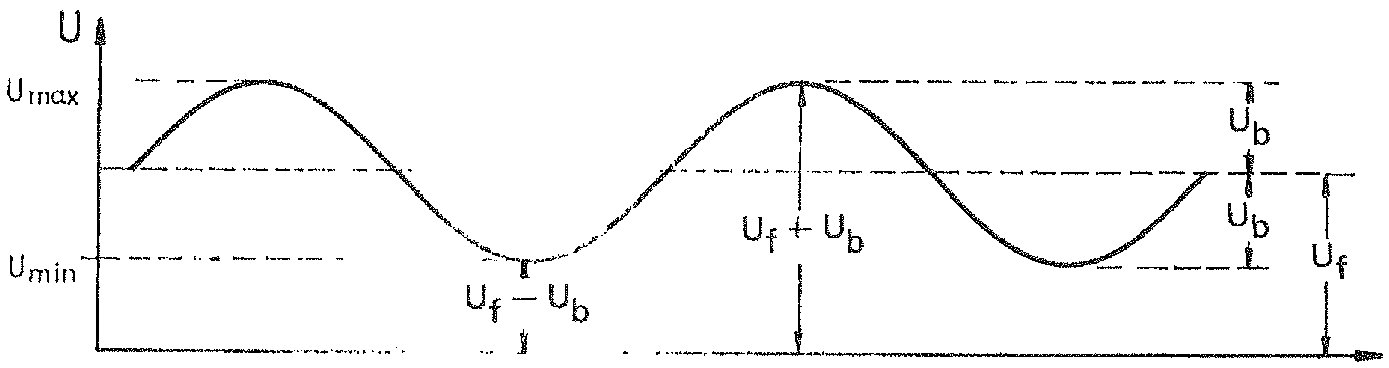
\includegraphics[width=\textwidth]{images/cropped_pdfs/bild_2_6-26.pdf}
  \caption{Stående våg på ledning}
  \label{fig:bildII6-26}
\end{figure}

Bild \ref{fig:bildII6-26} visar stående våg på ledning.
Spänningen utmed kabeln varierar regelbundet mellan

\[U_{max} = U_f + U_b \quad \text{och} \quad U_{min} = U_f - U_b\]

\subsection{Ståendevågförhållande (SVF)}
\textbf{
HAREC a.\ref{HAREC.a.6.3.6}\label{myHAREC.a.6.3.6}
}
\index{SVF}
\index{transmissionsledning!SVF}

(se även SWR = Standing Wave Ratio i avsnitt\ref{SVF}).

Med ståendevågförhållandet SVF menas förhållandet mellan \(U_{max}\)
och \(U_{min}\) eller mellan \(I_{max}\) och \(I_{min}\).

\begin{align*}
  \text{SVF} &= \frac{U_{max}}{U_{min}} = \frac{U_f + U_b}{U_f - U_b} \quad
  \text{eller} \\
  \text{SVF} &= \frac{I_{max}}{I_{min}}
\end{align*}

ståendevågförhållandet SVF kan även anges med hjälp av impedanserna i
matarledningen (\(Z\)) och i antennens matningspunkt (\(Z_a\)).

\begin{align*}
  \text{SVF} &= \frac{Z}{Z_a} \quad \text{där } Z > Z_a \quad \text{eller} \\
  \text{SVF} &= \frac{Z_a}{Z} \quad \text{där } Z > Z_a
\end{align*}

Ståendevågmätning beskrivs i avsnitt \ref{mäta ståendevåg}.

\begin{figure}
  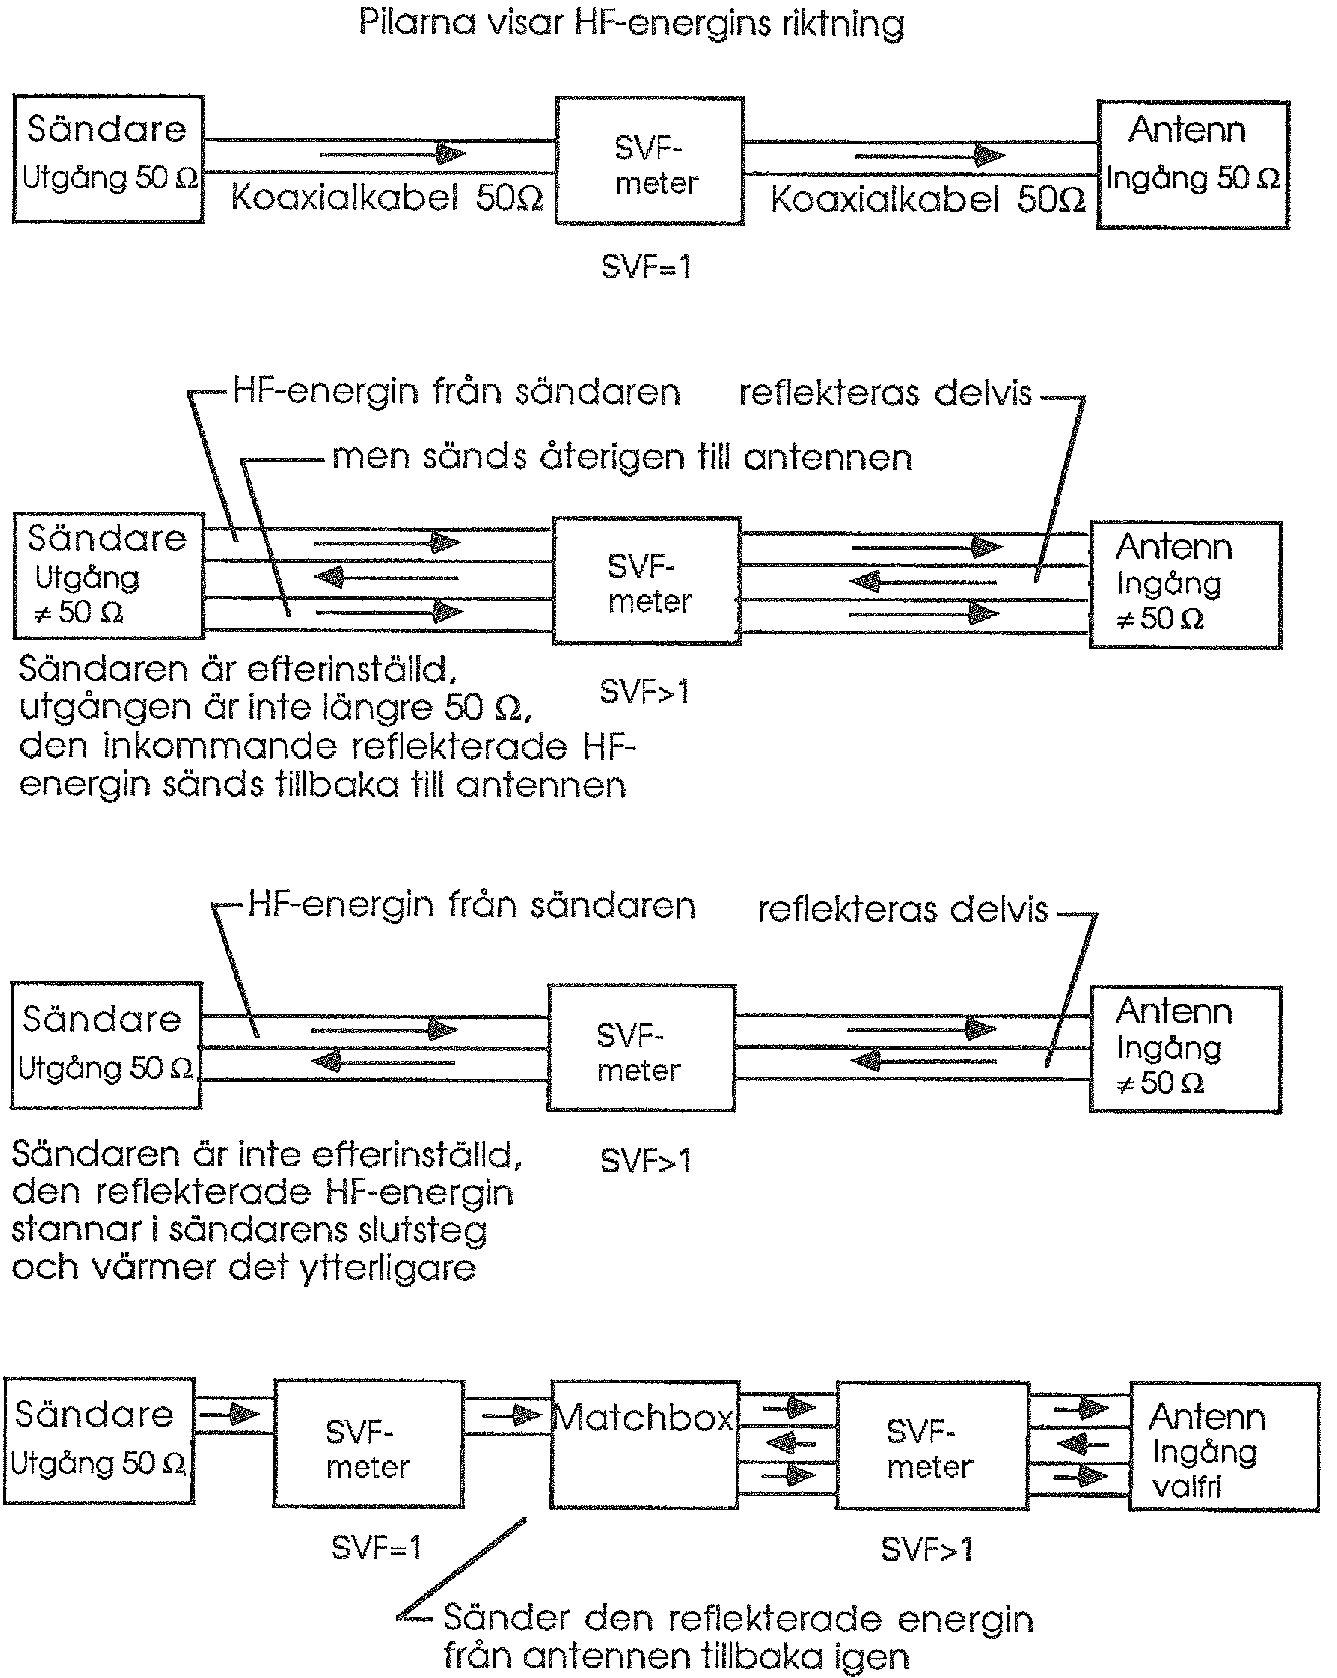
\includegraphics[width=\textwidth]{images/cropped_pdfs/bild_2_6-27.pdf}
  \caption{SVF-problemet förenklad bild}
  \label{fig:bildII6-27}
\end{figure}

Bild \ref{fig:bildII6-27} visar en förenklad bild av SVF-problemet och vad en
SVF-meter visar beroende på var den kopplas in i kedjan sändare -- ledning --
antennkopplare -- ledning -- antenn.

Vid ett högre SVF-tal än 2:1 till 3:1 vid sändarutgången, bör en antennkopplare
sättas in efter sändaren för att skydda den från (överhettning och) överslag.
Antennkopplare har även andra benämningar, t.ex. matchbox,
antennavstämningsenhet o.s.v.
Bäst är att göra sådana impedansanpassningar i alla led, att antennkopplaren
blir onödig.

\subsection{Effektförluster}
\textbf{
HAREC a.\ref{HAREC.a.6.3.7}\label{myHAREC.a.6.3.7}
}
\index{transmissionsledning!effektförlust}

I varje matarledning uppstår förluster, dels av resistansen i ledarna
och dels i isolationsmaterialet (dielektrikum) mellan ledarna samt i
någon mån av fältutstrålning från dem.
De mest påtagliga effektförlusterna i en ledning beror av förlusterna per
längdenhet och därmed även av längden.
Vidare beror förlusterna av ståendevågförhållandet på ledningen på grund av
dålig impedansanpassning.

Ett högt SVF-förhållande ger större ledningsförluster eftersom den
reflekterade effekten då pendlar fler gånger på ledningen.
Den reflekterade effekt som återvänder till ledningens början är mindre när
ledningen har stora förluster än om den inte hade det.
Det medför att det verkliga SVF-förhållandet i ledningens slut är
större än vad som syns på ett instrument i början.

Förlusterna i en transmissionsledning stiger med ökad frekvens och anges av
tillverkarna i datablad som dämpningen i dB per 100~m eller dB per 30~m ledning.

I tabell \ref{Kabeldämpning} visas kabeldämpningen, effektförlusten, i dB per
30~m för några vanliga typer av koaxialkablar.

\begin{table*}[!ht]
\begin{tabular}{|l|l|c|c|c|c|c|c|c|} \hline
	\text{Kabeltyp} & \text{Impedans} & 30 & 50 & 100 & 145 & 150 & 440 & 450 \\
	 & & \text{MHz} & \text{MHz} & \text{MHz} & \text{MHz} & \text{MHz} & \text{MHz} & \text{MHz}\\ \hline
	\text{RG8X} & 50 \text{ohm} & 2,0 & 2,1 & 3,0 & 4,5 & 4,7 & 8,1 & 8,6 \\ \hline
	\text{RG58A/U} & 50 \text{ohm} & 2,5 & 4,1 & 5,3 & 6,1 & 6,1 & 10,4 & 10,6 \\ \hline
	\text{RG59} & 75 \text{ohm} & & 2,4 & 3,5 & & & 7,6 & \\ \hline
	\text{RG174} & 50 \text{ohm} & 5,5 & 6,6 & 8,8 & 13,0 & & 25,0 & \\ \hline
	\text{RG213} & 50 \text{ohm} &  & 1,5 & 2,1 & 2,8 & 2,8 & 5,1 & 5,1 \\ \hline
	\text{RG214} & 50 \text{ohm} & 1,2 & 1,6 & 1,9 & 2,8 & 2,8 & 5,1 & 5,1 \\ \hline
\end{tabular}
\caption{Kabeldämpning per 30 m}
\label{Kabeldämpning}
\end{table*}

\subsection{Baluner -- Balansering -- Transformering}
\textbf{
HAREC a.\ref{HAREC.a.6.3.8}\label{myHAREC.a.6.3.8}
}

\subsubsection{Balansering}
\index{balun}

Man skiljer mellan symmetriska ledningar (bandkabel m.fl.) och osymmetriska
(koaxialkabel), där dessutom den ena ledaren (skärmen) ofta är jordad.

På samma sätt finns det symmetriska antenner (dipol, W3DZZ m.fl.) och
osymmetriska (ground plane, Marconi m.fl.).

Vill man ansluta en symmetrisk (mittmatad) antenn till en osymmetrisk
ledning (koaxialkabel), så måste en strömbalansering göras i övergången.
Om inte, så kommer matarledningen att stråla, vilket kan
medföra störningar på radio och TV.
Utan balansering kommer dessutom dipolens strålningsbild inte att vara
symmetrisk.

En balansering måste också göras i övergången mellan en bandkabel (symmetrisk)
och sändaren när den har anslutning för koaxialkabel (osymmetrisk).
Balansering av impedans och därmed ström sker med en
anordning kallad BAL UN (av de engelska orden BALanced-UNbalanced).

Baluner kan utföras på flera sätt.
Grundläggande har balunen lika in- och utgångsimpedans,

\textbf{Exempel:}

Ringkärnebalun 1:1 för balansering.

Koaxialledare anordnad som balun 1:1.

\subsubsection{Transformering}

\begin{wrapfigure}[23]{R}{0.5\textwidth}
  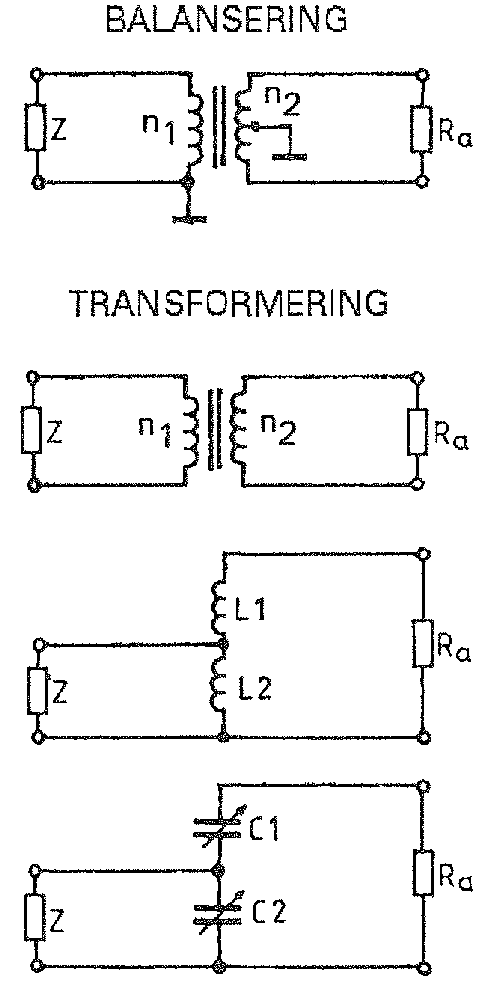
\includegraphics[width=0.5\textwidth]{images/cropped_pdfs/bild_2_6-28.pdf}
  \caption{Balansering -- transformering}
  \label{fig:bildII6-28}
\end{wrapfigure}

I samband med balanseringen kan en impedanstransformering behövas och det finns
baluner (transformatorer) som både balanserar och transformerar impedanser.

Bild \ref{fig:bildII6-28} visar en transformator med osymmetrisk ingång och
symmetrisk utgång.
Om båda lindningarnas varvtal är lika så sker ingen impedanstransformering.
Om förhållandet mellan varvtalen är 1:2 så blir förhållandet mellan
impedanserna 1:4. Se vidare i avsnitt \ref{transformator}.

Bilden visar också att matarledningens impedans \(Z\) transformeras om så
att den blir lika antennens anslutningsimpedans \(R_a\).
Dennatransformering kan ske induktivt eller kapacitivt.

\textbf{Exempel:}
Ringkärnebalun 1:4.

Koaxialledare anordnad som balun 1:4.

\subsection{Ringkärnebalun}
\index{balun!ringkärna}

Bild \ref{fig:bildII6-29} visar en \emph{ringkärnebalun} som är en form av
transformator.
I den finns en ringkärna av hårt sammanpressat järnpulver av en legering, som
tillsammans med lindningarnas utförande gör att frekvensbandbredden blir stor.

\begin{wrapfigure}{R}{0.5\textwidth}
  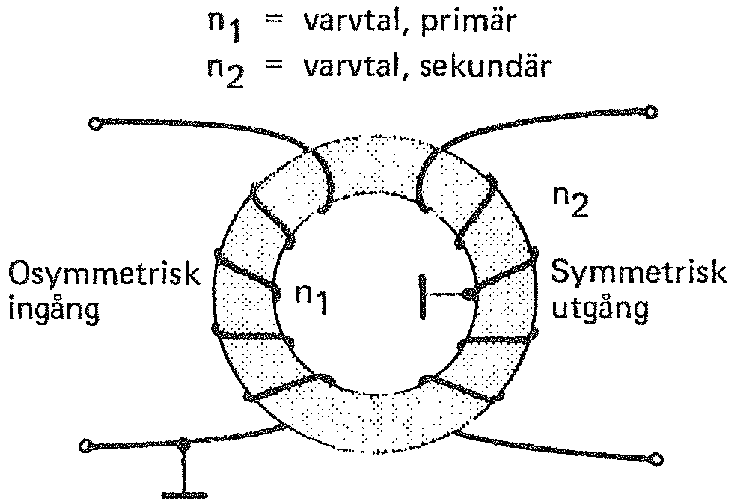
\includegraphics[width=0.5\textwidth]{images/cropped_pdfs/bild_2_6-29.pdf}
  \caption{Ringkärnebalun}
  \label{fig:bildII6-29}
\end{wrapfigure}

\subsection{Koaxialledare som balun}
\index{balun!koaxial}

Balansering kan även göras med ett ett koaxialkabelarrangemang, som i
så fall är starkt frekvensberoende.
Bild \ref{fig:bildII6-30} visar tre utföranden, som alla arbetar enligt
principen för en matarledning med en elektrisk längd av \(\lambda/4\) och
kortsluten i ena änden.

Den mekaniska längden är \(k\cdot\lambda/4\), varvid \(k\) är hastighetsfaktorn
för våghastigheten i kabeln.
För de vanligaste koaxialkablarna RG-58 och RG-213 är \(k\) ca 0,66.
\(\lambda/4\)-ledningen i den översta figuren fungerar som en
parallellsvängningskrets med mycket hög impedans \(Z\) i den öppna övre änden.

I den mellersta figuren är den översta delen av matningskabeln en
\(\lambda/4\) lång parallellsvängningskrets tillsammans med parallellt
ansluten ledare (i detta fall en koaxialkabel som kortslutits i båda ändar).
Den nedersta högra figuren i bilden visar den kortslutna
\(\lambda/4\)-ledningen i tre varianter.
I samtliga fall uppstår HF-mässigt en strömbalanserande effekt mellan
dipolhalvorna.

Dessutom hindras även antennströmmar från att komma ner på utsidan av
matningskabelns skärm

\begin{figure}
  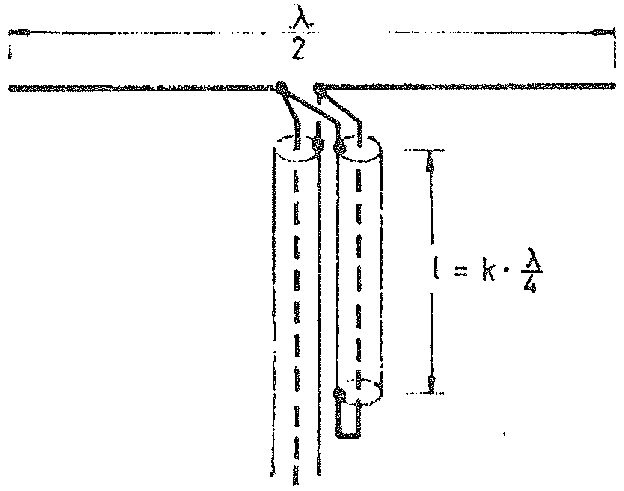
\includegraphics[width=0.5\textwidth]{images/cropped_pdfs/bild_2_6-30_1.pdf}
  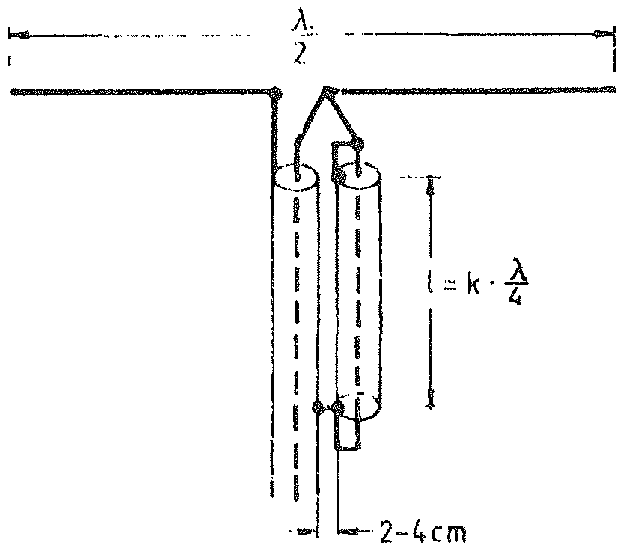
\includegraphics[width=0.5\textwidth]{images/cropped_pdfs/bild_2_6-30_2.pdf}
  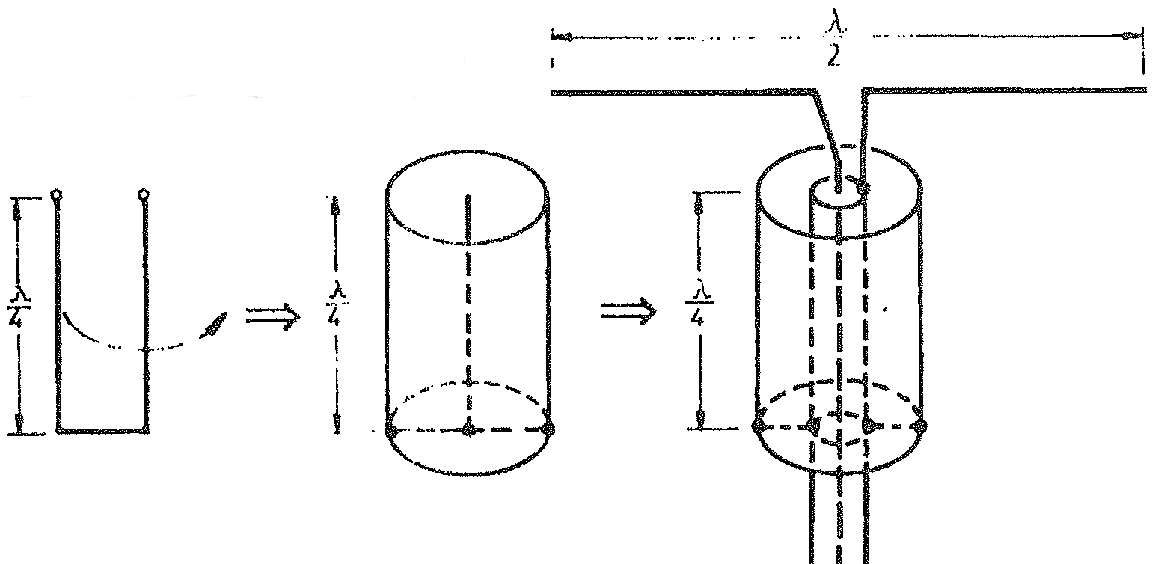
\includegraphics[width=\textwidth]{images/cropped_pdfs/bild_2_6-30_3.pdf}
  \caption{Koaxialledare som balun}
  \label{fig:bildII6-30}
\end{figure}

\begin{figure}
  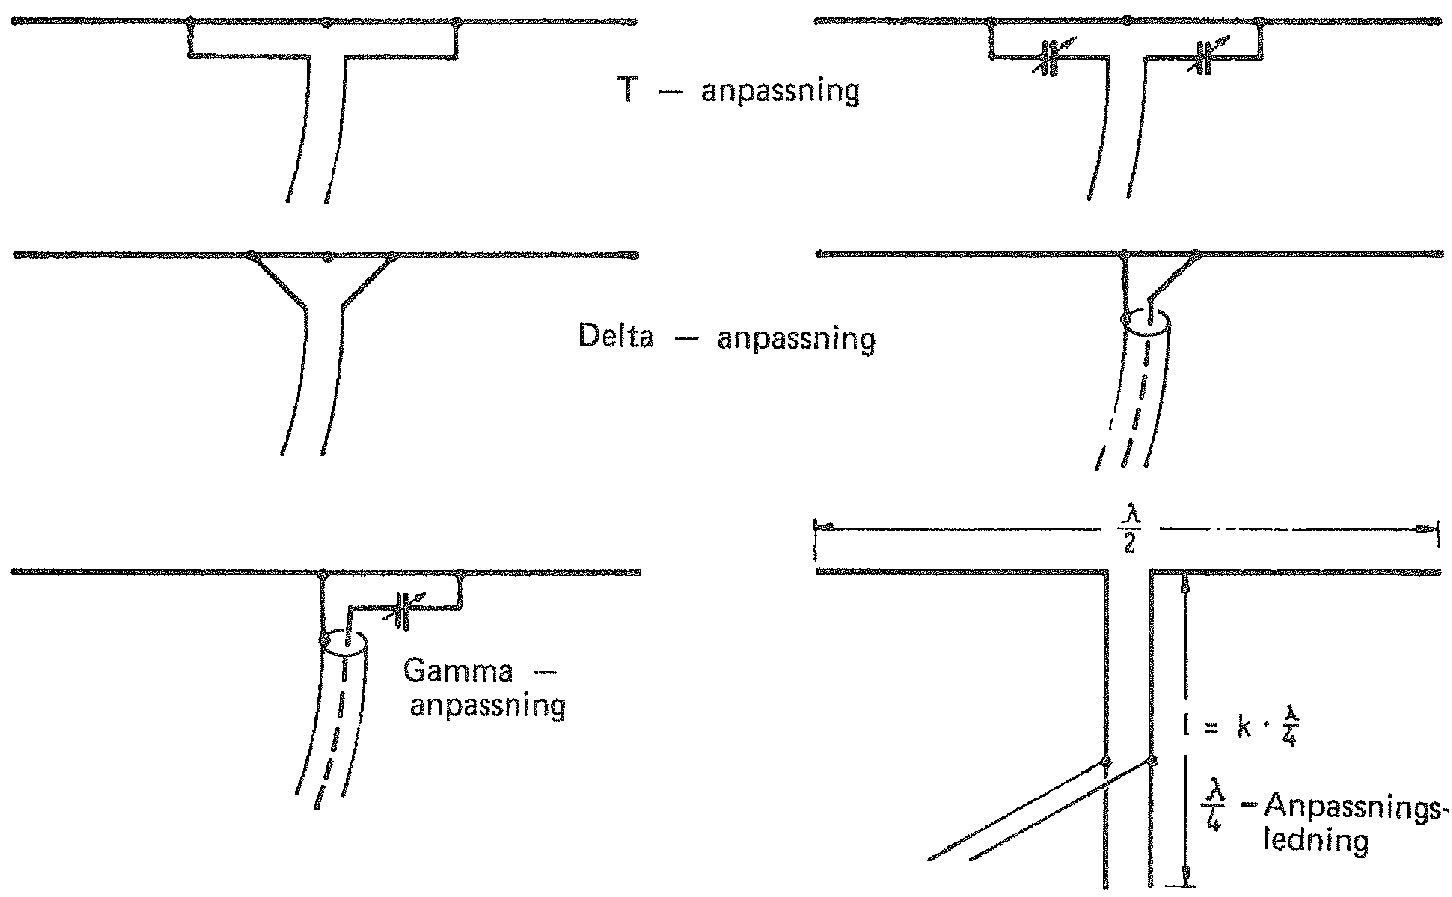
\includegraphics[width=\textwidth]{images/cropped_pdfs/bild_2_6-31.pdf}
  \caption{Sätt att ansluta en matningsledning}
  \label{fig:bildII6-31}
\end{figure}

\subsection{Sätt att ansluta en matningsledning}
\textbf{
HAREC a.\ref{HAREC.a.6.3.9}\label{myHAREC.a.6.3.9}
}
\index{antenn!anpassning}

Bild \ref{fig:bildII6-31} visar flera sätt att ansluta en matningsledning.

\subsubsection{T-, delta- och gamma-anpassning}

Funktion:
En mittmatad halvvågsdipol har i fria rymden en impedans av ca 73~\(\Omega\).

Flyttas matningspunkten bort från mitten, åt det ena eller andra
hållet, så är impedansen högre än i mitten.

Det finns alltid två symmetriskt liggande punkter på antennen där
impedansen är precis lika stor.

T-, delta- och gamma-anpassning är användbar när matarkabelns är högre
än antennens mittpunktsimpedans.
Matningsledningen kan anslutas till de punkter på antennen som har samma
impedans som matarledningen.
T-anpassning används för symmetriska matarledningar, gamma-anpassning för
osymmetriska ledningar och delta-anpassning för båda ledningstyperna.

\subsubsection{\(\lambda/4\)-anpassningsledning - stub}

Uppbyggnad: Antennen ansluts till en \(\lambda/4\) anpassningsledning
och matarledningen i sin tur till anpassningsledningen.

Funktion: Anpassningsledningen består av en öppen \(\lambda/4\)-matarledning.
Den har teoretiskt impedansen \(Z = 0\) den ände som är ansluten till antennen
och \(Z = \infty\) den andra.
Utmed anpassningsledningen finns alltid en impedans som är lika matarledningens
impedans.

\subsubsection{$\lambda/2$-fasningsledning}

\begin{wrapfigure}[13]{R}{0.5\textwidth}
  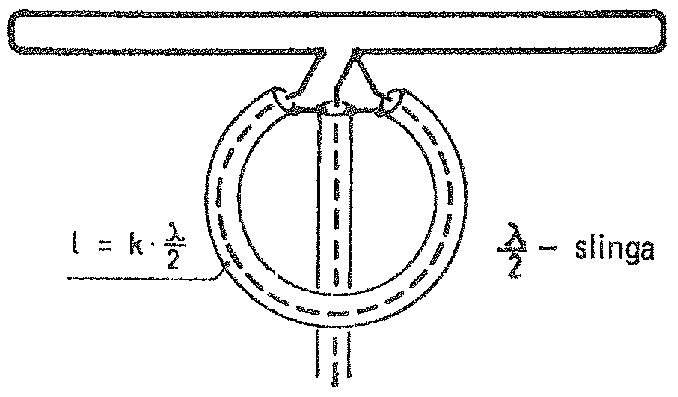
\includegraphics[width=0.5\textwidth]{images/cropped_pdfs/bild_2_6-32.pdf}
  \caption{$\lambda/2$-fasningsledning}
  \label{fig:bildII6-32}
\end{wrapfigure}

Bild \ref{fig:bildII6-32} visar en $\lambda/2$-fasningsledning.

Funktion: När t.ex. en omvikt dipol med matningsimpedansen 240~\(\Omega\) ska
anslutas till en 50~\(\Omega\)-kabel, behövs en impedanstransformering med
förhållandet 4:1.
En \(\lambda/2\) lång fasningsledning kan användas för detta ändamål.
Fasningsledningen har dessutom en strömbalanserande verkan.

Observera: Med en \(\lambda/2\)-fasningsledning enligt bilden kan
impedanstransformering endast göras i förhållandet 4:1.

\subsection{Transmissionsledningen}
\index{transmissionsledning}

En transmissionsledning för radiofrekvent energi består av två elektriska
ledare.
Den enklaste formen av en sådan ledning är två parallella ledare.
En annan form av transmissionsledning är koaxialkabeln, där den ena ledaren
löper inuti den andra.

Försök: Koppla en parallelledning till utgången på en VHF-sändare --
t.ex. med induktiv koppling.
Ge ledningen passande längd och mata ut högfrekvent energi på ledningen.
Nu kan fördelningen mellan spänning och ström på olika punkter utmed ledningen
undersökas.
När det finns en spänning mellan de två ledarna i ledningen alstras det ett
elektriskt fält mellan dem.

Eftersom en glimlampa lyser när den omges av ett elektriskt fält kan
den användas som en enkel spänningsindikator.
När en elektriskt ledande krets -- en induktionsslinga -- omges av ett
varierande magnetiskt fält alstras det en ström i slingan.
Med en glödlampa inkopplad i slingan kan den användas som en enkel
strömindikator.

\subsubsection{Öppen transmissionsledning}
\index{transmissionsledning!öppen}

\begin{figure}
  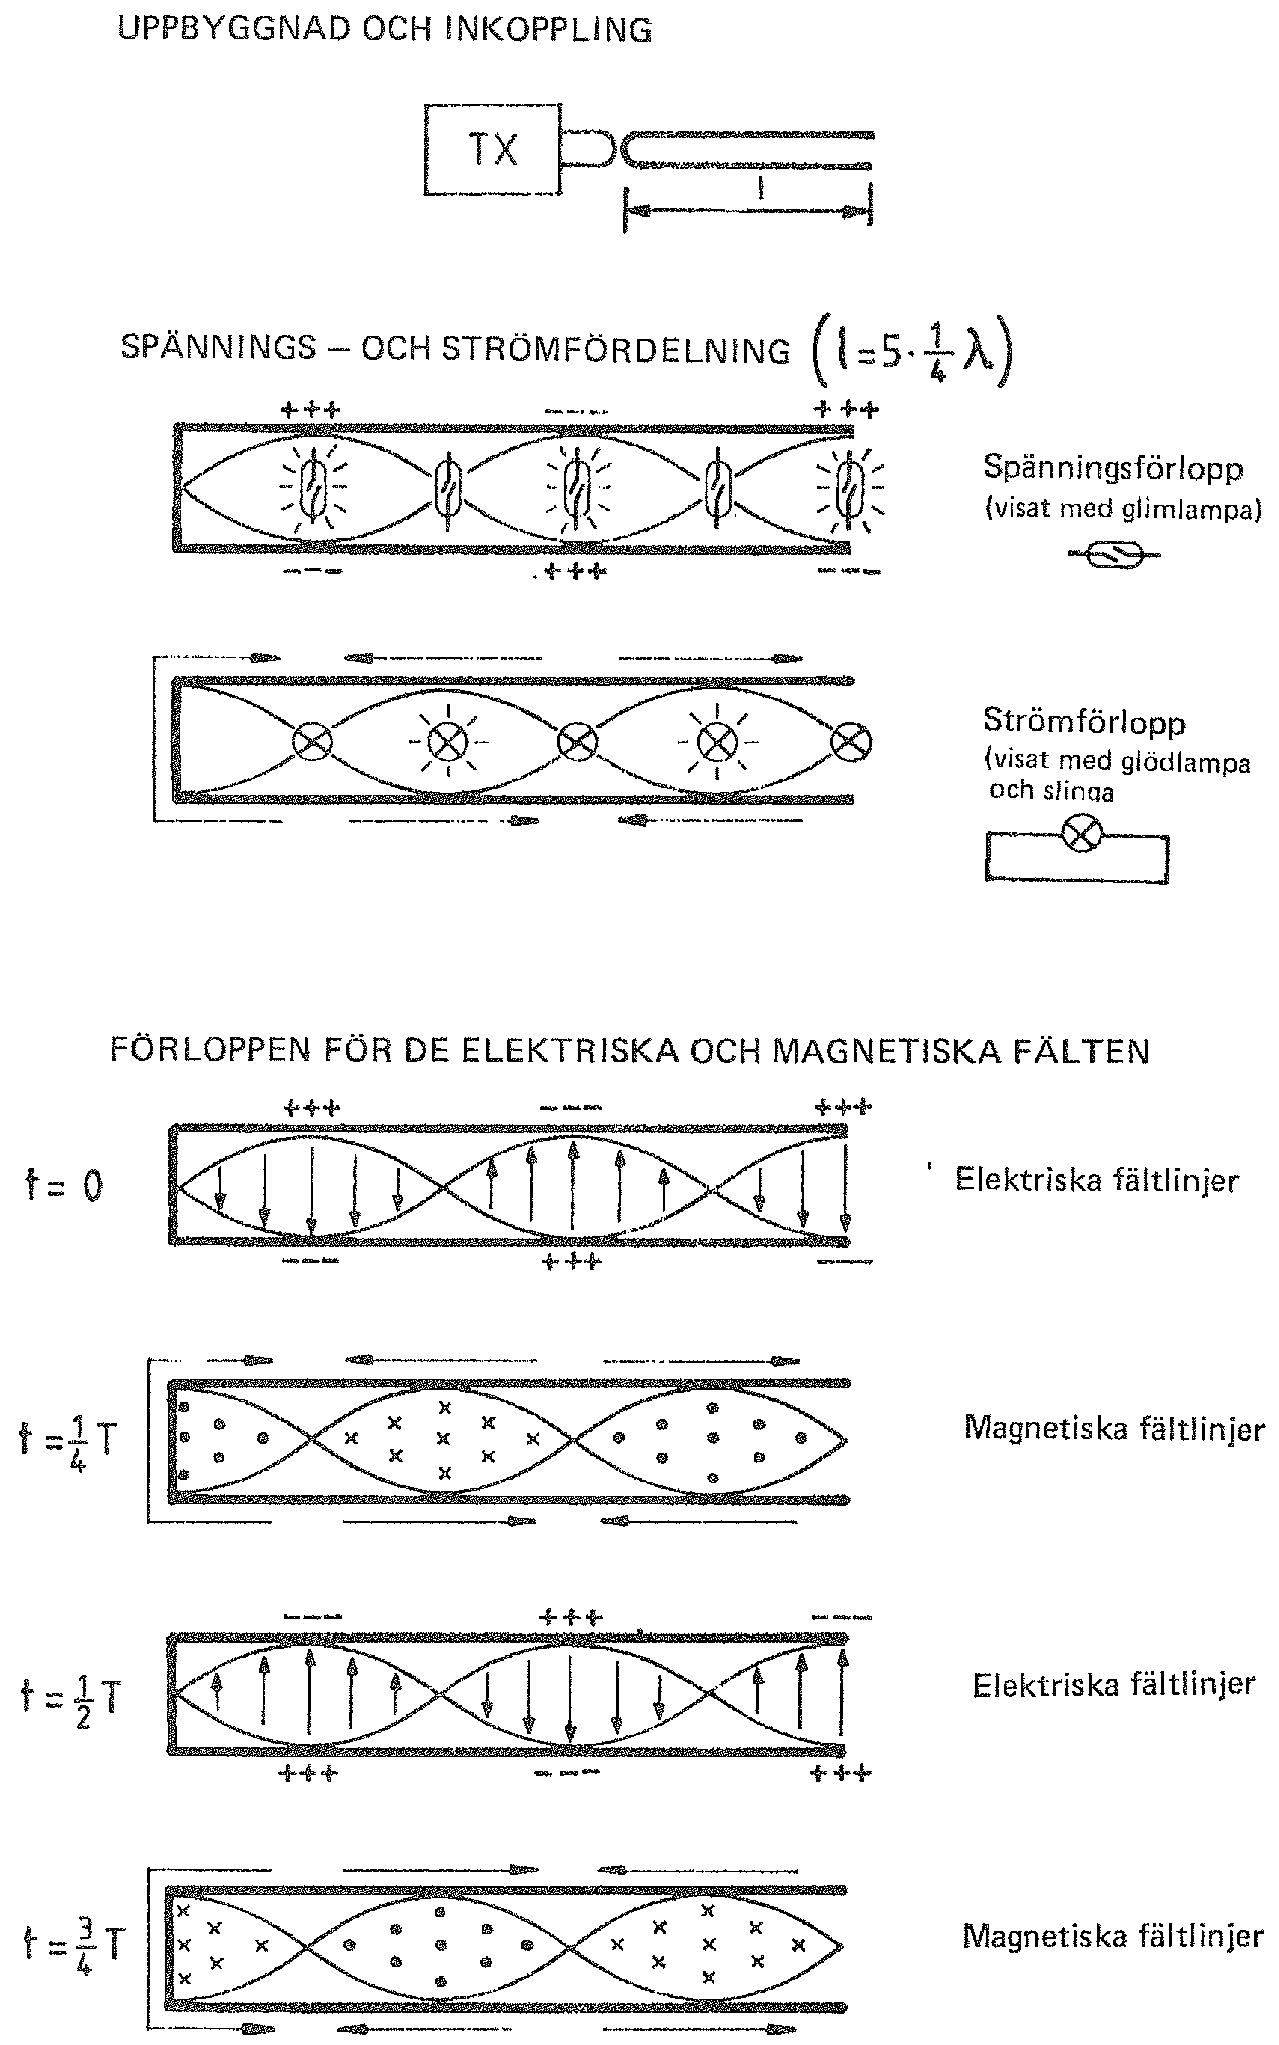
\includegraphics[width=\textwidth]{images/cropped_pdfs/bild_2_6-33.pdf}
  \caption{Förlopp i öppen $\lambda/4$ transmissionsledning}
  \label{fig:bildII6-33}
\end{figure}

Bild \ref{fig:bildII6-33} visar Förlopp i öppen $\lambda/4$
transmissionsledning.

Håll glimlampan nära intill ledningen.
Glimlampan tänds med jämna mellanrum när den flyttas utmed ledningen.

När i stället en induktionsslinga med glödlampa hålls nära intill ledningen,
kommer glödlampan att lysa mitt emellan de ställen där glimlampan lyser.
Där glimlampan tänder har det bildats spänningsmaximum och där glödlampan lyser
har det bildats strömmaximum.
Det har bildats en stående våg på ledningen.

Bilden visar ström- och spänningsfördelningen för en öppen transmissionsledning
med längden \(l = n\cdot\lambda/4\) med udda \(n = 1, 3, 5 \dots\).

För bilden har valts n = 5.

Utmed ledningen uppstår omväxlande elektriska och magnetiska fält allt
efter som svängningen fortsätter.
Med en serie om fyra figurer visas förloppet av en svängning, en period.
Skillnaderna i den elektriska fältstyrkan framställs som olika långa fältlinjer.
Observera fältlinjernas riktning.

Skillnaderna i den magnetiska fältstyrkan kan också utläsas ur
bilderna i form av antalet symboler ''\(\cdot\)'' respektive ''\(\times\)''.
Båda tecknen betecknar elektromagnetiskt fält, ''\(\cdot\)'' i riktning ut ur
papperet och ''\(\times\)'' in i papperet.
För tydlighetens skull skildras endast den elektromagnetiska fältstyrkan
mellan ledarna och inte utanför ledarparet.

\subsubsection{Kortsluten transmissionsledning}
\index{transmissionsledning!kortsluten}

\begin{figure}
  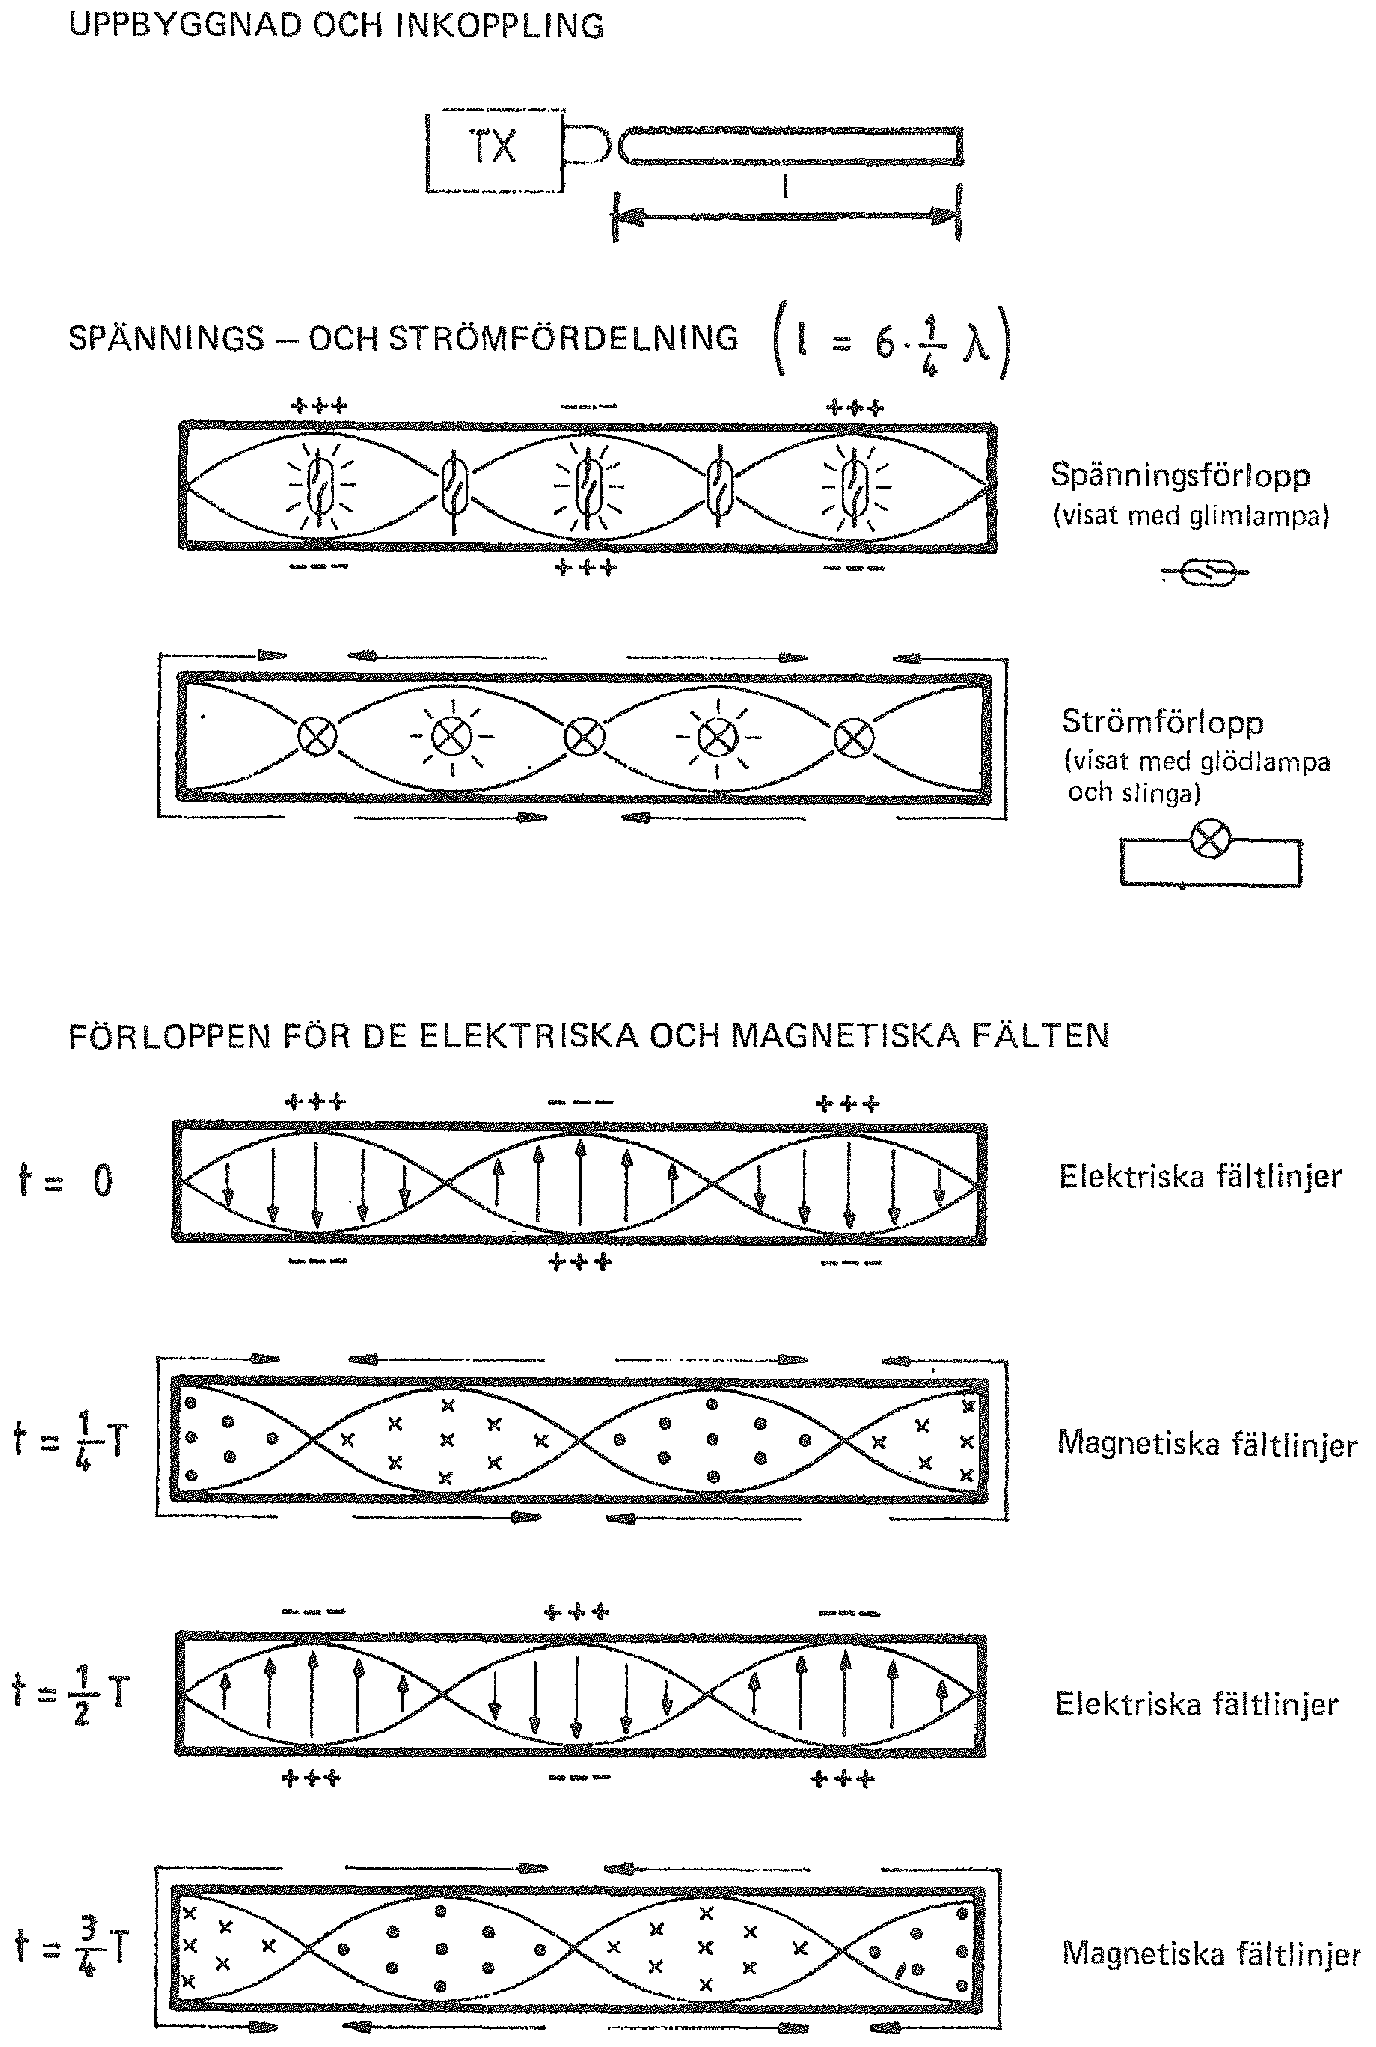
\includegraphics[width=\textwidth]{images/cropped_pdfs/bild_2_6-34.pdf}
  \caption{Förlopp i kortsluten $\lambda/4$ transmissionsledning}
  \label{fig:bildII6-34}
\end{figure}

På bild \ref{fig:bildII6-34} visas såväl ström- och spänningsförhållandena som
fältlinjeförloppen på en avstämd, kortsluten transmissionsledning med
längden \(l = \lambda/4\) med jämna \(n = 2, 4, 6, 8 \dots\).
För bilden har valts \(n = 6\).

\subsection{$\lambda/4$-ledning som svängningskrets}

\begin{figure}
  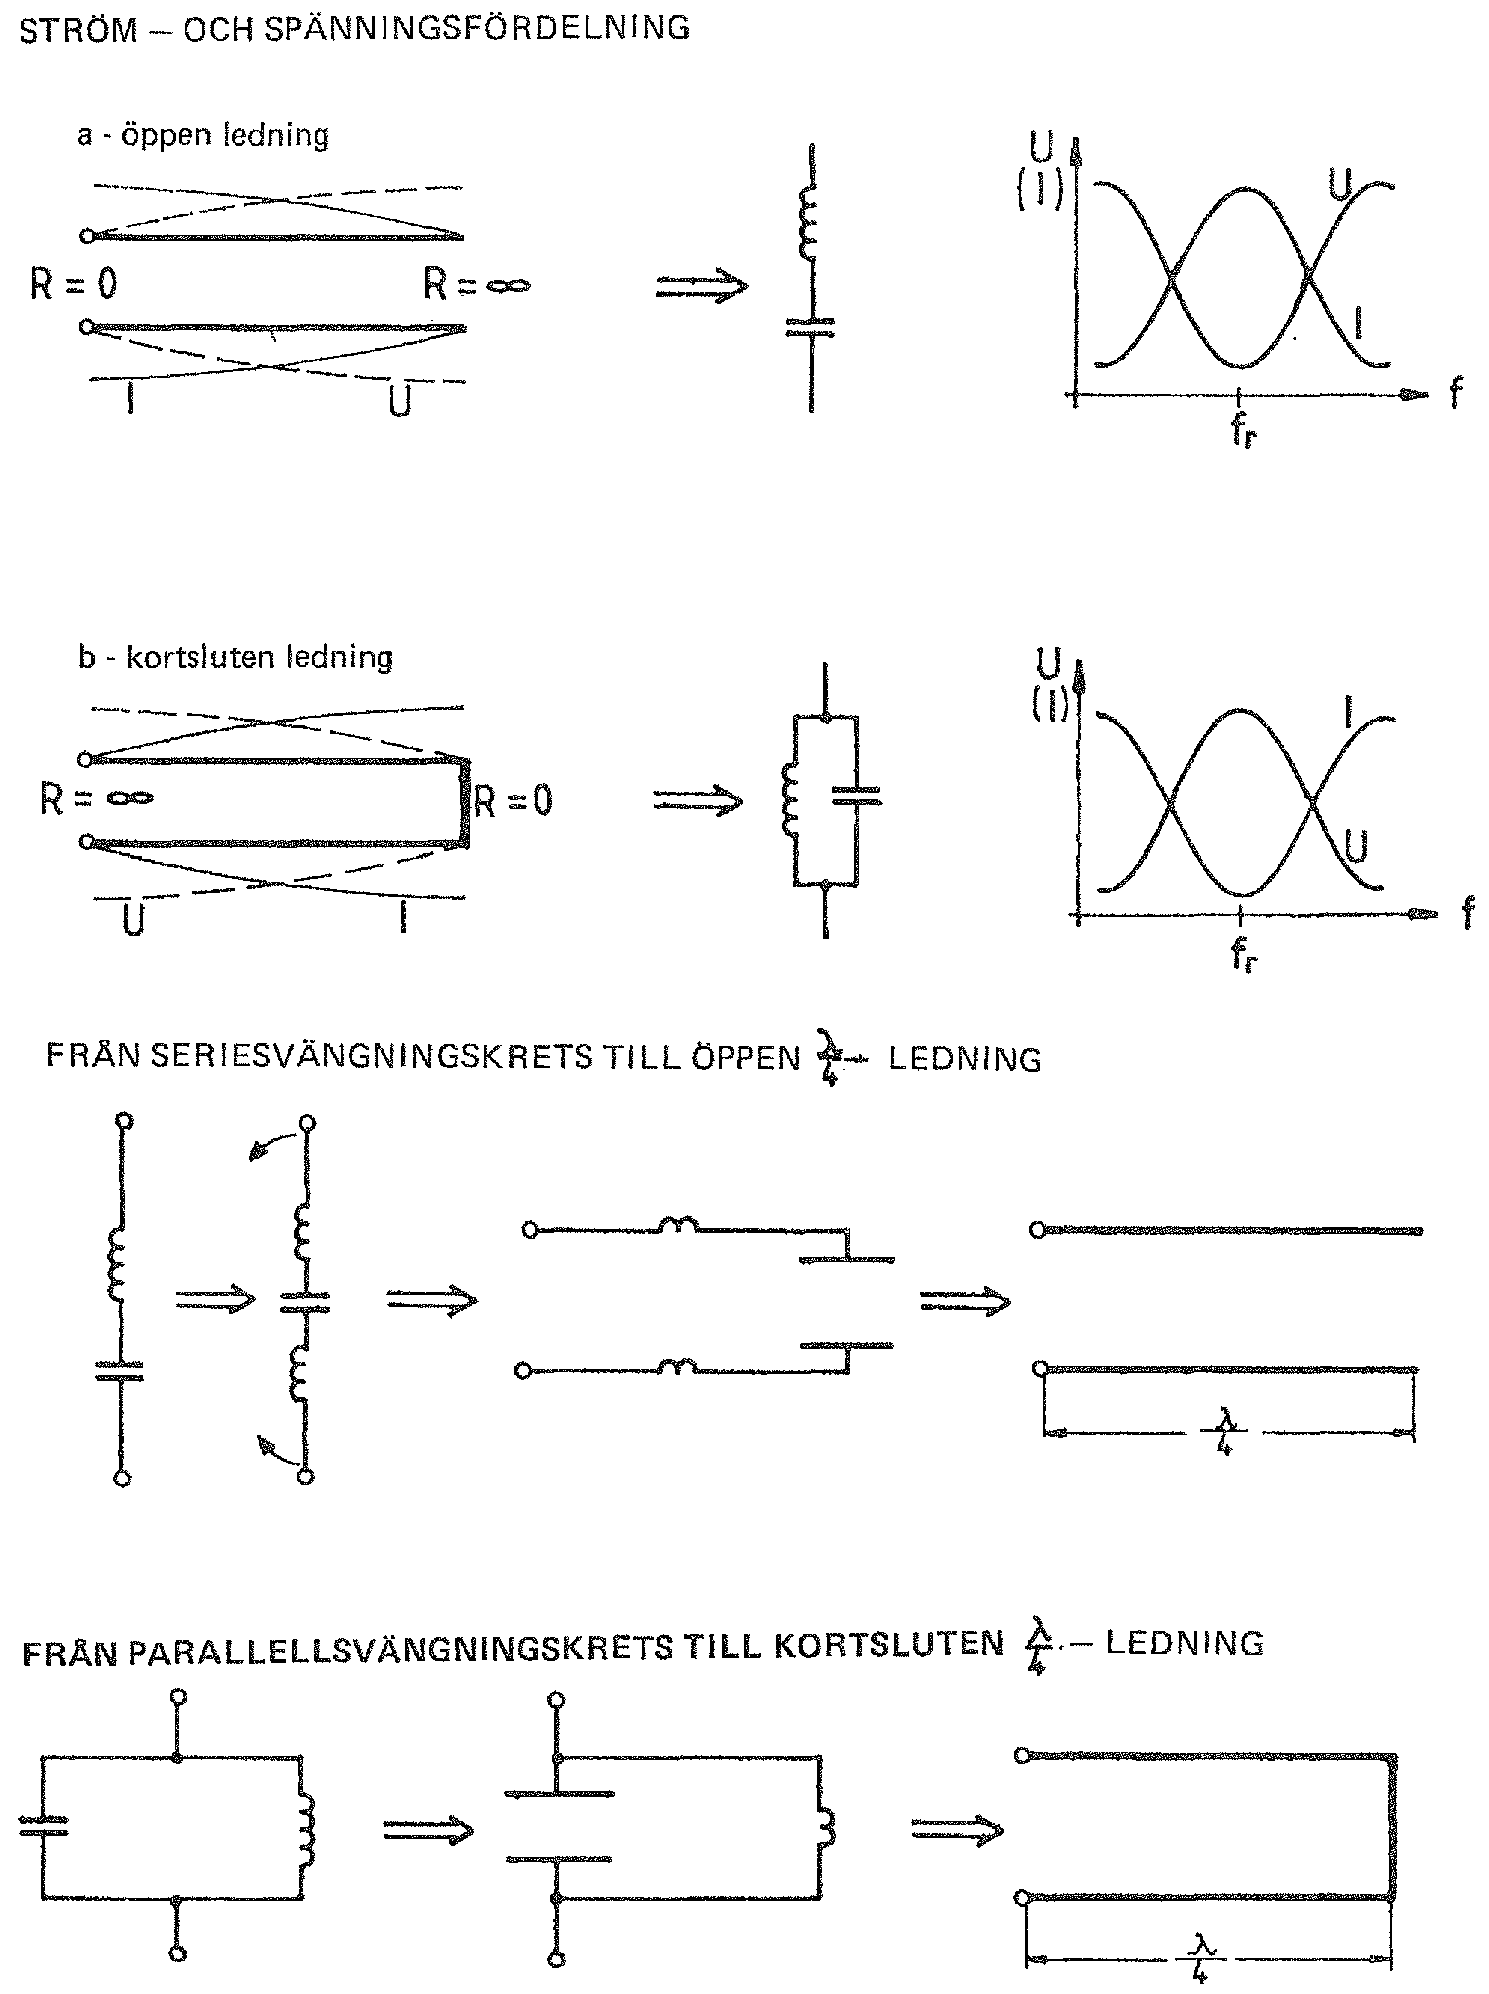
\includegraphics[width=\textwidth]{images/cropped_pdfs/bild_2_6-35.pdf}
  \caption{$\lambda/4$ transmissionsledning som svängningskrets}
  \label{fig:bildII6-35}
\end{figure}

Bild \ref{fig:bildII6-35} visar ström- och spänningsfördelningen för en öppen
resp. en kortsluten transmissionsledning med längden \(l = \lambda/4\).

Den öppna \(\lambda/4\)-ledningen har en strömbuk i ingångsänden.
En sådan ledning måste således strömkopplas, d.v.s. den anslutande
impedansen måste vara låg.

Den kortslutna \(\lambda/4\)-ledningen har en spänningsbuk i ingångsänden.
En sådan ledning måste spänningskopplas, d.v.s. den anslutande impedansen måste
vara hög.

En öppen \(\lambda/4\)-ledning kan ses som en seriekopplad LC-krets.
När ledningen är i resonans flyter en hög ström i ingången, medan spänningen
där är låg.

En kortsluten \(\lambda/4\)-ledning kan ses som en parallellkopplad LC-krets.
När ledningen är i resonans är spänningen hög över ingången, medan strömmen där
är låg.

\clearpage % Fulhack för att undvika att bild 6-36 inte ska hamna tre sidor bort från subsection
%
\begin{wrapfigure}[35]{R}{0.5\textwidth}
  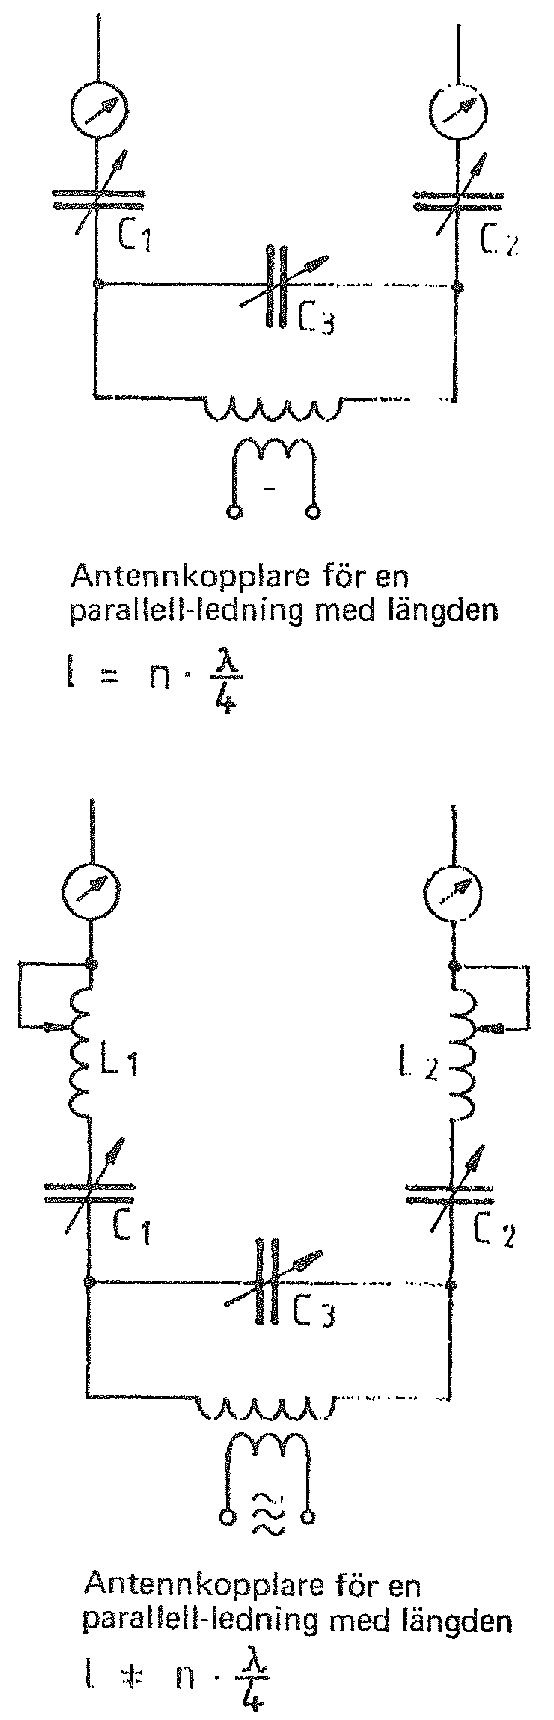
\includegraphics[width=0.5\textwidth]{images/cropped_pdfs/bild_2_6-36.pdf}
  \caption{Antennkopplare}
  \label{fig:bildII6-36}
\end{wrapfigure}
%
\subsection{Antennkopplare}
\index{antenn!anpassning}

Bild \ref{fig:bildII6-36} visar en antennkopplare för bandkabel av olika
längder. Storleken på kondensatorerna: \(C_1 = C_2 = 500\text{ pF},
C_3 = 300\text{ pF}\).

\subsubsection{Avstämning vid spänningskoppling}
\index{antenn!avstämning}

\(C_1\) och \(C_2\) helt invridna eller kortslutna, \(C_3\) avstäms
för resonanstillstånd (parallellresonans).

\subsubsection{Avstämning vid strömkoppling}

\(C_3\) helt utvriden, \(C_1\) och \(C_2\) avstäms för
resonanstillstånd (serieresonans), med maximal och lika ström i båda ledarna.

Matarledningen kan förlängas elektriskt med induktanser när den är för
kort för att kunna avstämmas.

Märk, att en antennkopplare mycket väl även kan utformas för
koaxialkabelutgång.

\subsection{För- och nackdelar med avstämd matarledning}

När en matarledning är rätt avstämd transporterar den energi utan att
stråla själv.

När dipolen kopplas till en avstämd matarledning, kan den med hjälp av
en antennkopplare arbeta på flera amatörradioband.
Detta är en anledning till varför en avstämd matarledning gärna används för
portabla installationer (t.ex. för field days).
Injusteringen mot sändaren blir enklare.

Inom amatörradion används numera nästan uteslutande koaxialkabel som
matarledning i stället för bandkabel.
Detta är av flera skäl:

\begin{itemize}
\item En bandkabel måste hängas upp så fritt som möjligt och den får
  inte komma för nära murutsprång, takrännor o.s.v.
  Vidare måste den isoleras väl vid genomföringar i väggar.

\item De flesta sändaramatörer har inte plats med långa matarledningar
  (\(n\cdot\lambda/4\) med \(n = 1, 2, 3 \dots\)).

\item Vid tvära bockar på ledningen kan det upp stå oönskad
  utstrålning och därmed risk för störningar på radio och TV m.m.

\end{itemize}
